%%%%%%%%%%%%%%%%%%%%%%%%%%%%%%%%%%%%%%%%%%%%%%%%%%%%%%%%%%%%%%%%%%%%%%%%%%%%%%
\section{TS1 collar}

Figure~\ref{figure:vd4_muons_vs_pbars_1037} shows Y:X distribution at VD4 for
muons and antiprotons stopping in the ST.

\begin{figure}[H]
  \begin{tikzpicture}
    \node[anchor=south west,inner sep=0] at (0,0.) {
      % \node[shift={(0 cm,0.cm)},inner sep=0,rotate={90}] at (0,0) {}
      \makebox[\textwidth][c] {
        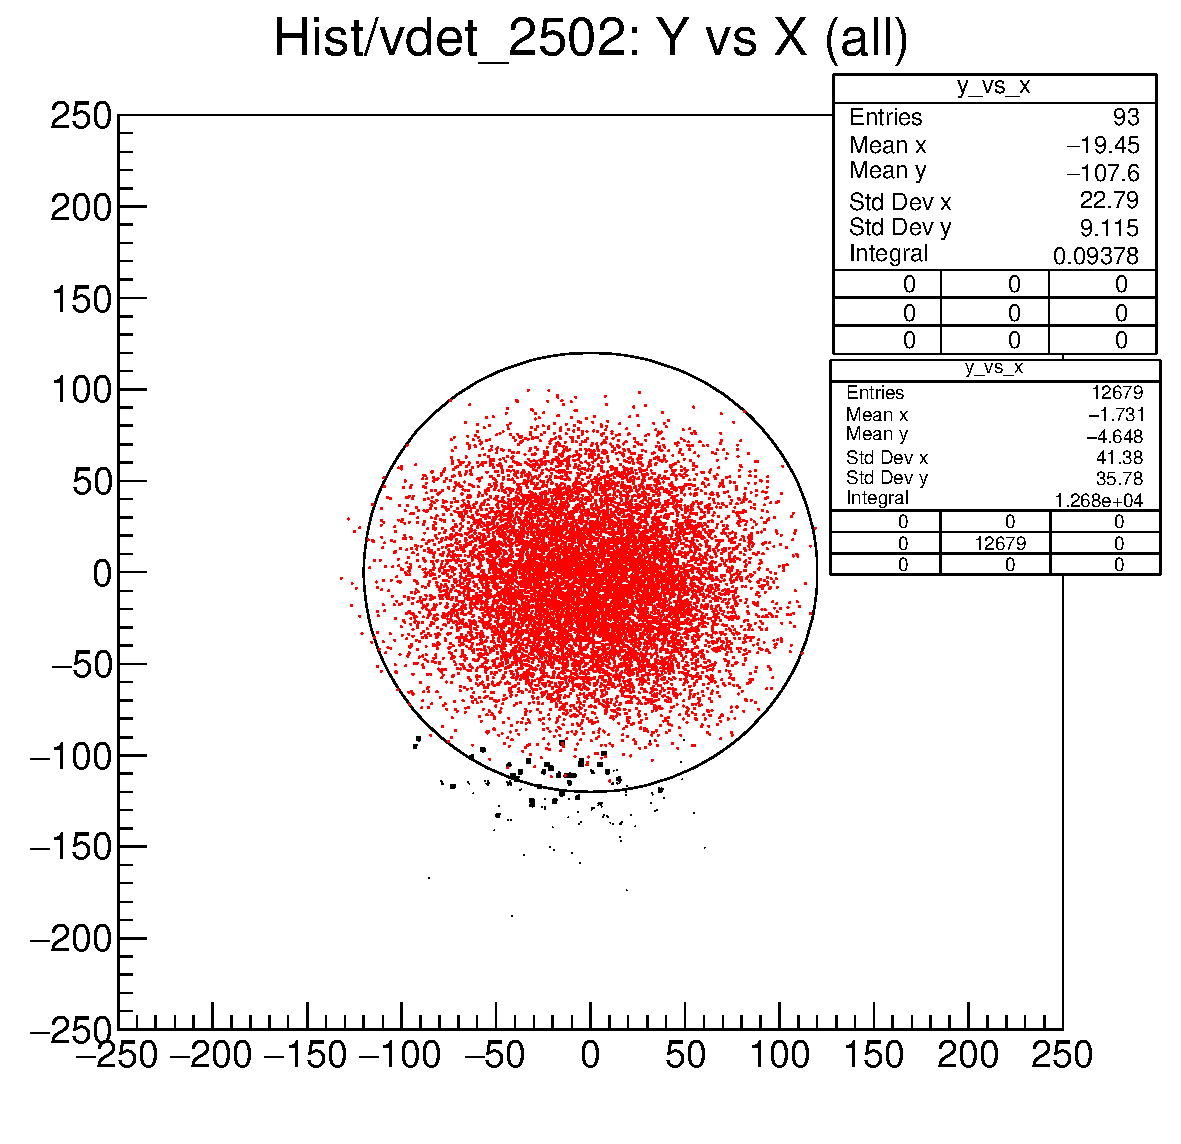
\includegraphics[width=0.5\textwidth]{figures/pdf/vd4_muons_vs_pbars_1037}
      }
    };
    % \node [text width=6cm, scale=0.8] at (4.5,6.4) {mu2e-18894 by Kevin Lynch and Jim Popp};
  \end{tikzpicture}
  \caption{
    \label{figure:vd4_muons_vs_pbars_1037}
    aaa
  }
\end{figure}

As pbars are concentrating on the bottom, placing a ``collar'' on the bottom of TS1 
reduces the pbar flux out of TS1 by a factor of several.

For TS1 window of 250 um Al, and TS3 win: 200um Ti, 1x14cm x 127um Al strip in 3 yr:
expected background, with and without the collar: 0.15 vs 0.03 events in 3 years of running

\begin{figure}
  \begin{tikzpicture}
    \node[anchor=south west,inner sep=0] at (0,0.) {
      % \node[shift={(0 cm,0.cm)},inner sep=0,rotate={90}] at (0,0) {}
      \makebox[\textwidth][c] {
        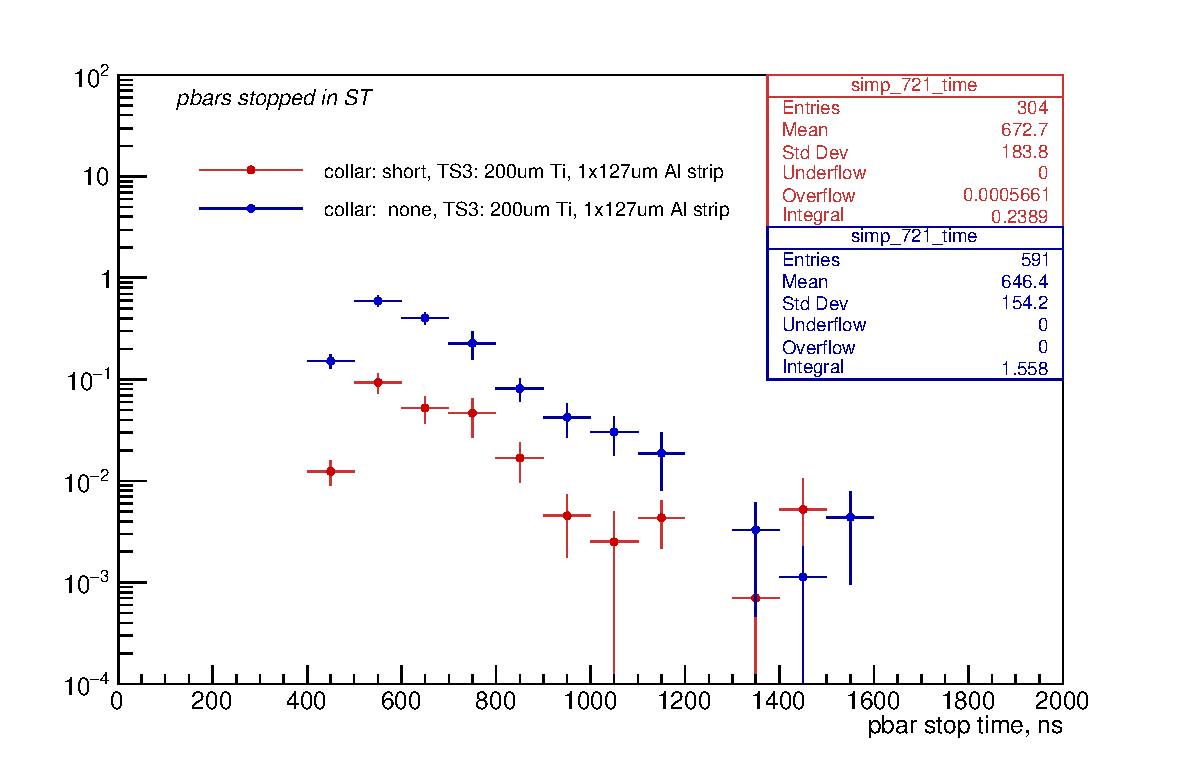
\includegraphics[width=0.8\textwidth]{figures/pdf/760_1022_vs_760_4022_ts4_tgtstops_simp_721_time}
      }
    };
    % \node [text width=6cm, scale=0.7] at (4.5,6.4) {mu2e-18894 by Kevin Lynch and Jim Popp};
  \end{tikzpicture}
  \caption{
    \label{figure:760_1022_vs_760_4022_ts4_tgtstops_simp_721_time}
    aaa
  }
\end{figure}

Within the acceptance, TS1 collar suppresses antiprotons of all momenta, with the suppression efficiency
increasing with momentum.

\begin{figure}
  \begin{tikzpicture}
    \node[anchor=south west,inner sep=0] at (0,0.) {
      % \node[shift={(0 cm,0.cm)},inner sep=0,rotate={90}] at (0,0) {}
      \makebox[\textwidth][c] {
        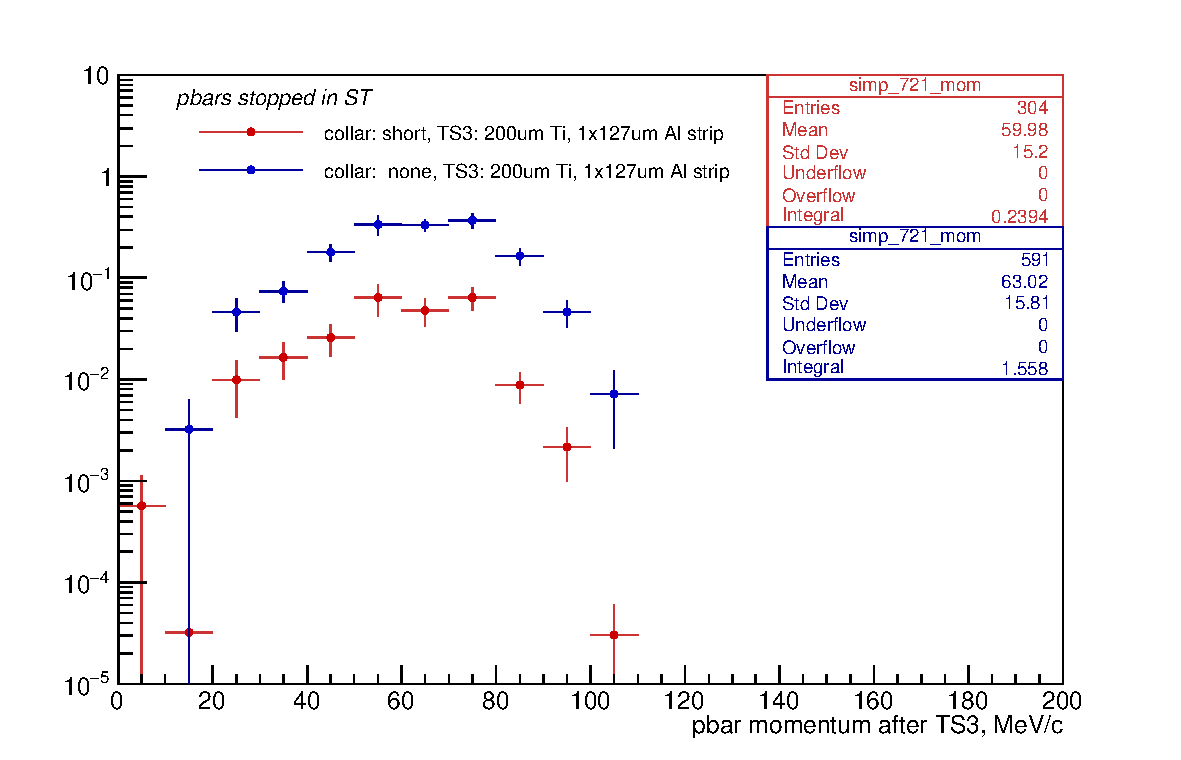
\includegraphics[width=0.8\textwidth]{figures/pdf/760_1022_vs_760_4022_ts4_tgtstops_simp_721_mom}
      }
    };
    % \node [text width=6cm, scale=0.8] at (4.5,6.4) {mu2e-18894 by Kevin Lynch and Jim Popp};
  \end{tikzpicture}
  \caption{
    \label{figure:760_1022_vs_760_4022_ts4_tgtstops_simp_721_mom}
    aaa
  }
\end{figure}




%%% Local Variables:
%%% mode: latex
%%% TeX-master: t
%%% End:
